\documentclass[11pt,letterpaper]{article}

\usepackage{textcomp}
\usepackage{amsfonts}
\usepackage{verbatim}
\usepackage[english]{babel}
\usepackage{pifont}
\usepackage{color}
\usepackage{setspace}
\usepackage{lscape}\parskip=6pt
\usepackage{tabu}
\usepackage{booktabs}
\usepackage{multirow}

\usepackage{gensymb} % You have to have this to use \degree
\usepackage{float}
\usepackage{latexsym}
\usepackage{hyperref} 
\usepackage{url}
% Reference Supp labels
% \usepackage{zref-xr}
\usepackage{epsfig}
\usepackage{graphicx}
\usepackage{amssymb}
\usepackage{amsmath}

\usepackage{caption}
\usepackage{lineno}
\usepackage[utf8]{inputenc}
\usepackage{sectsty,setspace,natbib}
\usepackage[top=1.00in, bottom=1.0in, left=1in, right=1in]{geometry}
\usepackage{graphicx}
\usepackage{latexsym,epsf,rotating}
\usepackage{epstopdf}
\usepackage{todonotes}

\linespread{1.2} % was 1.66 for double-spaced 
% \raggedright
\setlength{\parindent}{0.5in}

\setcounter{secnumdepth}{0}

\pagestyle{empty}

\renewcommand{\tableofcontents}{}


\pagenumbering{arabic}
\pagestyle{plain}


\usepackage{fancyhdr}

\begin{document}
\linenumbers
\bigskip
\medskip
\begin{center}

% Insert your title:
\noindent{\Large Trophic phenological mismatch: Disconnects between underlying ecological theory and climate change responses} 
\bigskip

\noindent {\normalsize \sc
H.M. Kharouba $^{1}$ \& E.M. Wolkovich$^{2}$}\\
\bigskip
\noindent {\small \it
$^1$ Department of Biology, University of Ottawa, Ottawa, ON, Canada, K1N 9B4\\
$^2$ Forest \& Conservation Sciences, Faculty of Forestry, University of British Columbia, 2424 Main Mall, Vancouver, BC V6T 1Z4}\\

\end{center}
\bigskip
\noindent Corresponding author: H.M. Kharouba, e-mail: heather.kharouba@uottawa.ca.\\

\noindent \textbf{Running Title:}\\
\noindent \textbf{Keywords:} phenology, climate change, variety, diversity, resilience\\ 
\noindent \textbf{Type:} Ideas \& Perspectives

\section{Abstract}
Climate change's warming seasons and shifting precipitation regimes have impacted winegrowing regions across the globe: grapes are harvested earlier, alcohol has increased and recent years have seen lower yields in some regions. Here we review how the $>1,000$ different varieties grown today could help regions adapt. These varieties possess tremendous diversity in their responses to climate, yet most exist only in the Old World, with New World regions growing fewer varieties and planting most hectares with only 1\% of the total diversity. We discuss ways to better exploit this diversity and understand which varieties will be ideal in coming decades. 




\section{Introduction}

Climate change is causing phenological shifts (i.e. changes in the timing of life history events) that vary across species in different functional groups and trophic levels \citep{ovaskainen2013,caradonna2014, thackeray2016}. Such species-specific variation in response to climate change has led to changes in the relative timing of key activities (phenological synchrony) among interacting species \citep{kharouba2018}. These changes have caused fitness consequences—often termed ‘phenological mismatch’ (Box 1)—and have influenced ecosystem-level properties in some contexts \citep{post2007, burkle2013, plard2014, doiron2015} but not others \citep{vatka2011, burthe2012}. Predicting phenological mismatches will be key for determining the extent to which pair-wise species interactions, communities, and ecosystem function (e.g. pollination) will be affected by climate change. Despite many theoretical \citep{johansson2015,bewick2016} and empirical studies (REF) based in single systems, we still have no general ability to predict the outcomes of shifts in phenological synchrony due to climate change.  \par

Here, we argue that much of the difficulty in predicting the consequences of climate change-driven shifts in synchrony is due to a disconnect between ecological theory and current empirical approaches in the phenological mismatch literature. Current methodological inconsistencies across studies make it difficult to test the relevant underlying ecological theory in the context of climate change. Without better evidence, we cannot attribute variation in findings across studies to species, site, or mechanism. Without an understanding of the mechanisms underlying the well-documented patterns in phenological shifts, our ability to make accurate predictions about species’ responses, and species’ interactions, to climate change remains limited \citep{oconnor2012, chmura2018}. \par

Here, we focus on the widely-cited Cushing match-mismatch, or trophic mismatch, hypothesis \citeyearpar{cushing1974}, the most commonly applied hypothesis to consumer-resource interactions in this literature. We show how advances could come from direct tests of the hypothesis and clear definitions of baselines, when possible. Our aim is not to put forward additional hypotheses about the context in which phenological mismatch will occur, which has been reviewed extensively elsewhere \citep[e.g.,][] {millerrushing2010}, Renner and Zohner 2018), but rather to help guide the study of phenological mismatch to develop more robust predictions.  \par

Although the Cushing hypothesis has been applied to other types of interactions (e.g. mutualism), we limit our discussion to consumer-resource interactions (i.e. antagonistic). Below, we provide an overview of the Cushing hypothesis, summarize our literature review of phenological mismatch and then outline the divide between the hypothesis and the empirical studies. We discuss how current approaches are impeding major progress in the field but that changes in our approach could rapidly advance our understanding and help forecast of the impacts of climate change on ecological communities, the ultimate goal of most of the phenological mismatch literature. \\

%\subsection
\noindent \emph{Overview of the main ecological theory}\\

The most common ecological theory that underlies phenological mismatch studies (Appendix) is the Cushing match-mismatch hypothesis. This hypothesis predicts the often-shown concave down curve between consumer fitness and relative timing between the consumer and its resource \citep[;Figure 1]{cushing1974}. While this curve has been applied across many ecosystems (CITES), the theory originally emerged from the marine fisheries literature as a way to explain the variation in population recruitment of fish stocks. 

\section{Disconnect between theory and empirical studies}
In its original state, the hypothesis has been debated, contested and criticized, particularly in the marine literature (Durant et al. 2007, Leggett and DeBlois 1994*). In part because, although a relatively simple hypothesis, it is inherently difficult to test in the field, an assertion even Cushing himself made. Indeed, the shape and strength of the relationship of the curve varies greatly across observational studies (e.g., Philippart et al. 2013; Reed et al. 2013; Plard et al. 2014; Atkinson et al. 2015). While others have suggested that this is because of data limitations and the model’s implication of complex multitrophic dynamics (Kerby chapter, Durant et al. 2007), we argue that there are key methodological reasons that make it difficult to determine whether this hypothesis is widely supported in the context of climate change. Below, we introduce the current objectives of the phenological mismatch literature, and then discuss how studies often fail to rigorously test the Cushing hypothesis. We also examine whether studies define pre-climate change baselines, which are critical for assessing climate change impacts now, and in the future.

\subsection{Testing fundamental theory}

The Cushing hypothesis offers a testable, generally applicable hypothesis for predicting the magnitude and direction of demographic changes in response to climate-change driven shifts in synchrony (Figure 2). To date, much research in the biological impacts of climate change literature has focused on the direct relationships between organisms and the environment (e.g., Menzel et al. 2006, Chen et al. 2011) rather than testing theory (Lavergne et al. 2010; O’Connor et al. 2012; Mouquet et al. 2015; Barner et al. 2018). However, progress on the Cushing hypothesis requires tests of a diversity of ecological and evolutionary theory. This represents the major challenge of the hypothesis and—we argue—may be why support for it has been so mixed. 

%=======================================================================
\section{Acknowledgements}
%=======================================================================

%=======================================================================
% References
%=======================================================================

\bibliography{mismatch2}
\bibliographystyle{apa}

%=======================================================================
% Tables
%=======================================================================
\newpage
%\section{Tables}
\begin{table}[ht!]
\caption{A comparison across studies of the type of performance data collected for consumer and resource.  We define a life-history study as one that collected data at the individual level and a food-web study as one that collected data at the population or community (i.e., across species) level data}
\begin{center}
\resizebox{6.5in}{!}{
\begin{tabular}{ c c c c c c c c } % a table with 8 columns
\toprule
\multicolumn{3}{c}{}& \multicolumn{5}{c}{Resource performance}\\
\cmidrule{4-8}
\multicolumn{3}{c}{}& & Life-history & \multicolumn{2}{c}{Food-web} &\\
\cmidrule{5-7}
\multicolumn{3}{c}{} & None & Individual & Population & Community & Totals\\
\midrule 
\multirow{4}{*}{Consumer performance}&Life-history & Individual & 7 & 0 & 4 & 14 & 25\\
\cmidrule{2-8}
 & \multirow{2}{*}{Food-web}& Population & 2 & 1 & 7 & 7& 17\\
 \cmidrule{3-8}
 & & Community & 0 & 0 & 1 &1 & 2\\
 \cmidrule{2-8}
 & & Totals & & & & & 44\\ 
 \bottomrule 
\end{tabular}
}
\end{center}
\end{table}
\clearpage
%$$$$$$$$$$$$$$$$$$$$$$

%\section{Tables}
\begin{table}[ht!]
\caption{A comparison across studies of the type of performance data collected for the consumer across systems and taxonomic group}
\begin{center}
\resizebox{6.5in}{!}{
\begin{tabular}{ c c c c c c c c } % a table with 8 columns
\toprule
\multicolumn{2}{c}{}& \multicolumn{2}{c}{System} & \multicolumn{4}{c}{Taxonomic group}\\
\cmidrule{3-4} \cmidrule{5-8}
\multicolumn{2}{c}{}& Aquatic & Terrestrial & Invertebrate & Fish & Bird & Mammal\\
\midrule 
\multirow{4}{*}{Consumer performance}& Individual & 6 & 20 & 1 & 2 & 15 & 6\\
\cmidrule{2-8}
 & Population & 13 & 3 & 9 & 4 & 2 & 1\\
 \cmidrule{2-8}
 & Community & 1 & 1 & 2 & 0 & 0 & 0\\
 \cmidrule{2-8}
 & Totals & 20 & 24 & 12 & 6 & 17 &7\\ 
 \bottomrule 
\end{tabular}
}
\end{center}
\end{table}
\clearpage

%=======================================================================
% Figures
%=======================================================================
%^^^^^^^^^^^^^^^^^^^^^^^^^^^^^^^^^^^^^^^^^^^^^^^^^^^^^^^^
\begin{figure}[ht!]
\caption{Simple conceptualization of the Cushing curve; with climate change predictions.}
\begin{center}
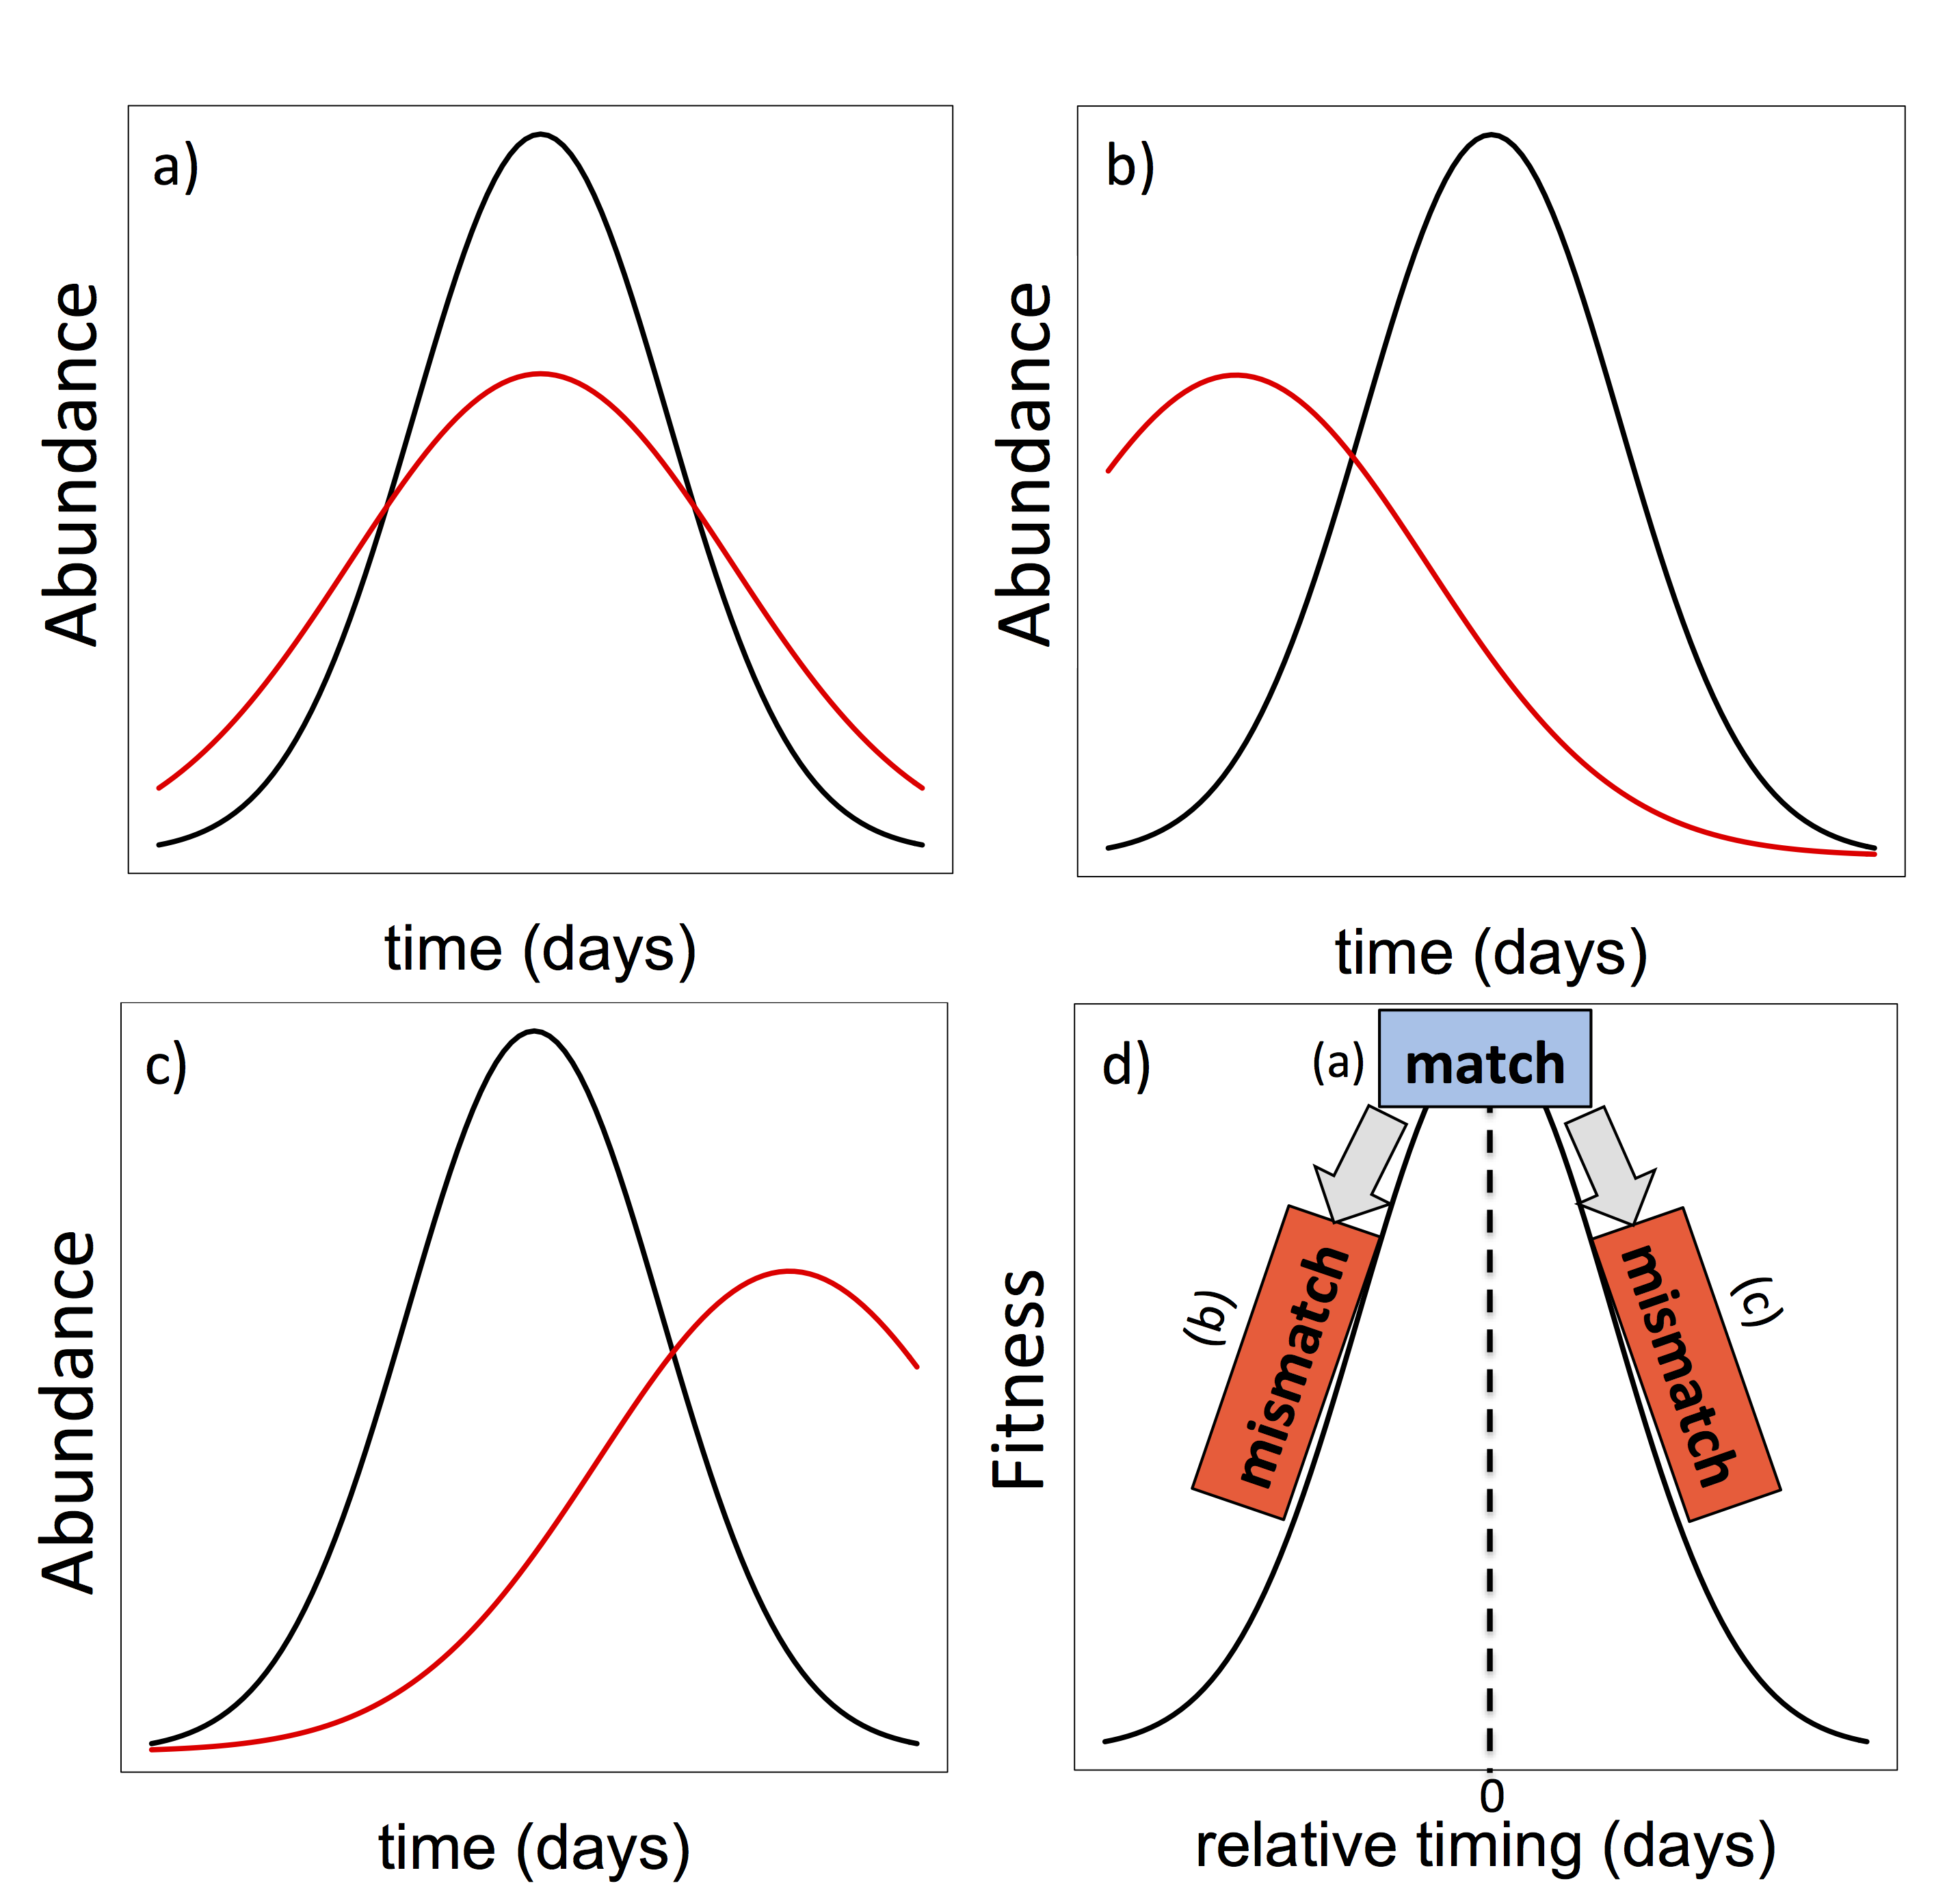
\includegraphics[width=0.9\textwidth]{fig1_v1.png}
\end{center}
\end{figure}
\clearpage
%^^^^^^^^^^^^^^^^^^^^^^^^^^^^^^^^^^^^^^^^^^^^^^^^^^^^^^^^

\begin{figure}[ht!]
\caption{Stationarity and change with climate change (a); then assumed max fitness, pre-climate change baseline (b); alternative baselines (c) … note this means (b) does not have the shallow curve from Singer \& Parmesan 2010, but c would, yielding two examples of the major alternatives: (1) you’re on a different spot on the curve that max fitness before climate change and (2) the curve is different.}
\begin{center}
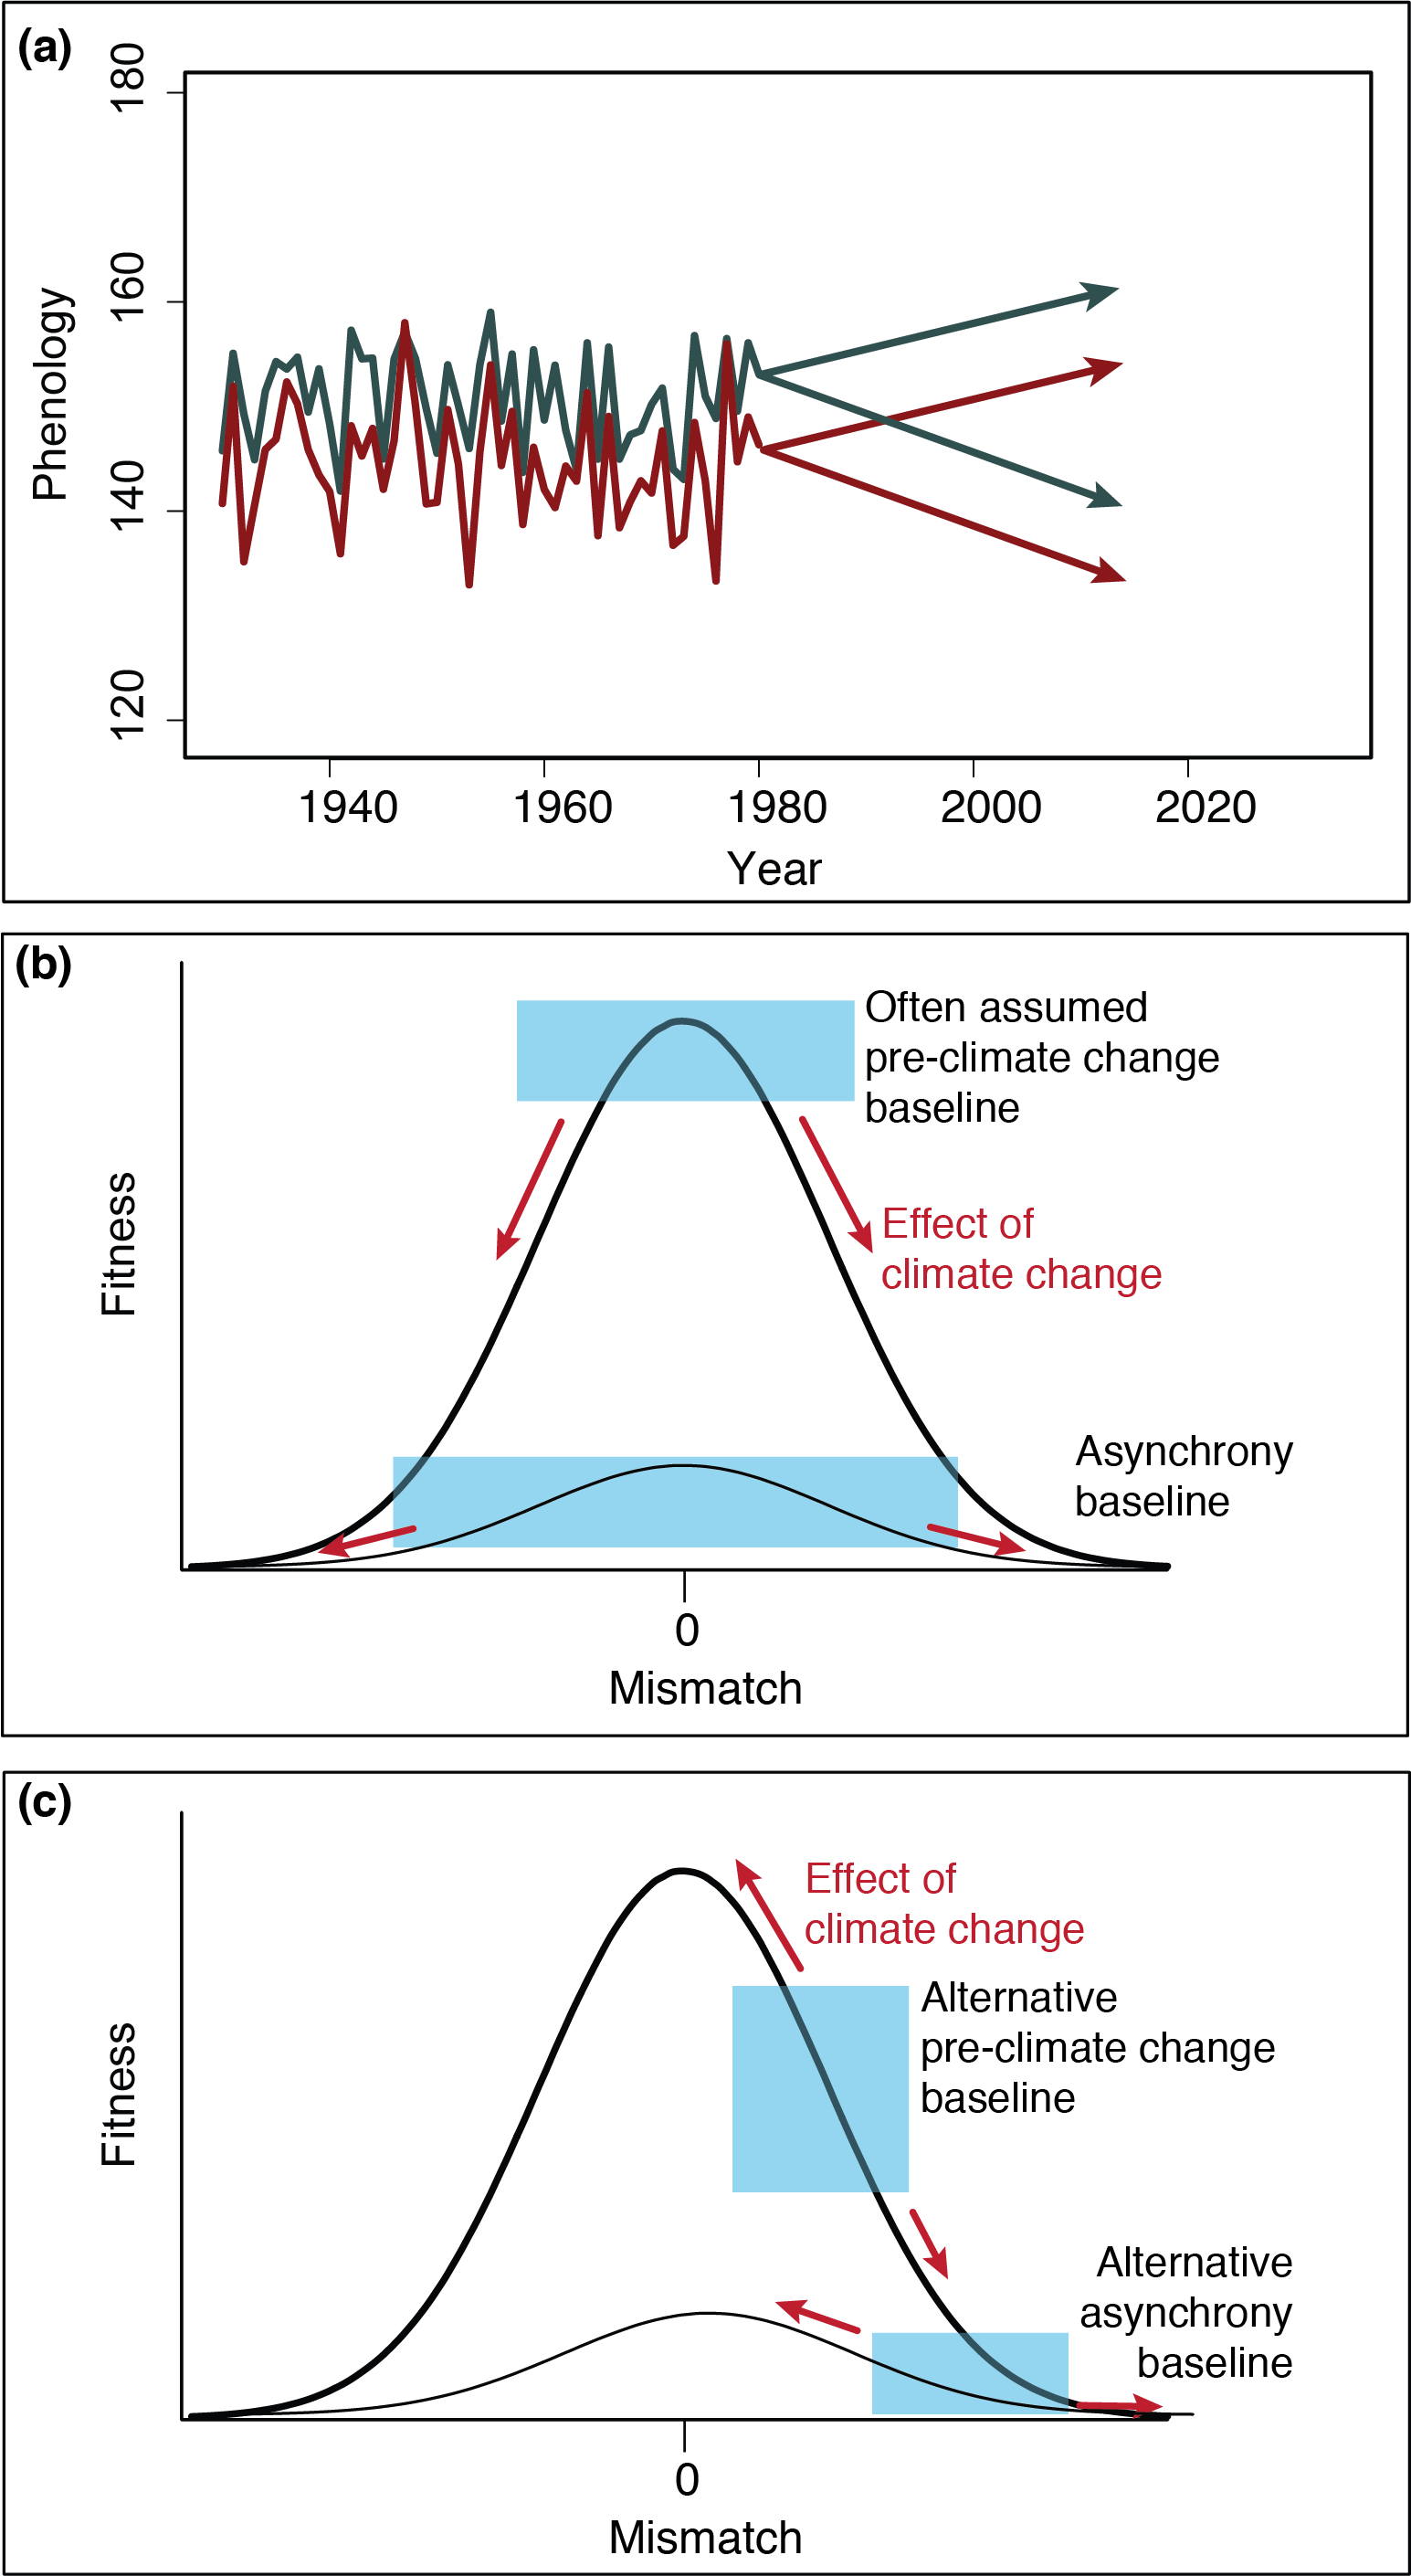
\includegraphics[width=0.65\textwidth]{fig2.png}
\end{center}
\end{figure}
\clearpage

%^^^^^^^^^^^^^^^^^^^^^^^^^^^^^^^^^^^^^^^^^^^^^^^^^^^^^^^^

\begin{figure}[ht!]
\caption{Case study demonstrating the integration of experimental (a) and observational data (b) relating to the Cushing hypothesis in a single system- the winter moth (Operophtera brumata) and oak (Quercus robur). (a) Experimental raw data was obtained from Tikkanen and Julkunen-Tiitto (2003) and result from two experiments (green, red points). In the first experiment, the authors manipulated the number of days that neonates (i.e. early instar larvae) spent without food (green points). In the second experiment, they manipulated the emergence times of larvae. There were four cohorts, each separated by intervals of 3-5 days. All O. brumata eggs originated from laboratory stock originally from Turku, Finland whereas the foliage originated from trees near Banchory, NW Scotland. (b) Inter-annual variation in relative timing between median egg hatch date of O. brumata and the median bud opening date of Q. robur from 1996-2005 in the Netherlands. Horizontal error bars represent the lower and upper quartiles of the data. Raw data from the observational study was retrieved from VanAsch and Visser 2007 Figure 2. In this system, negative values along the x-axis denote where egg hatching occurred before bud opening, whereas positive values indicate egg hatching occurred after bud opening.}
\begin{center}
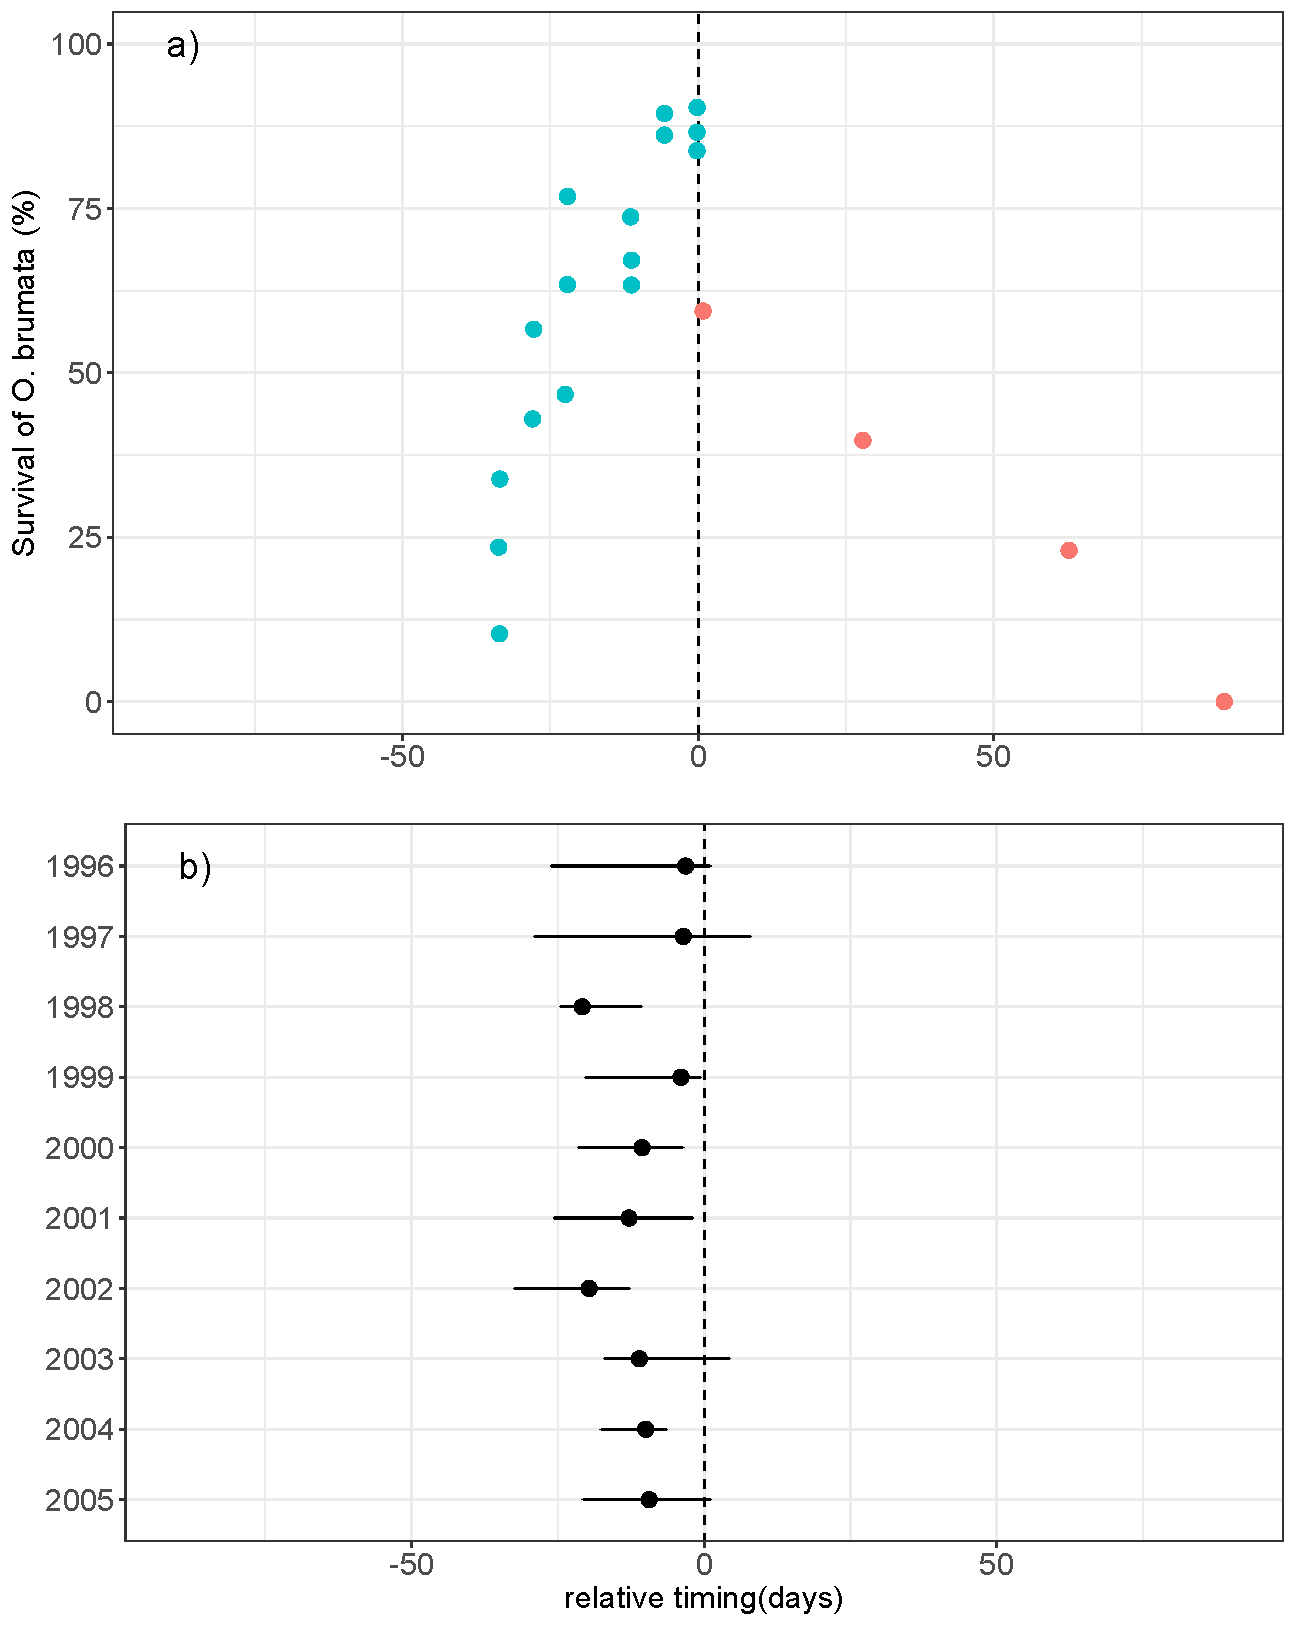
\includegraphics[width=0.8\textwidth]{fig3_v1.png}
\end{center}
\end{figure}
\clearpage

%^^^^^^^^^^^^^^^^^^^^^^^^^^^^^^^^^^^^^^^^^^^^^^^^^^^^^^^^

%\end{flushleft}
\end{document}  